% Typeset with LaTeX format
% Using AMS extensions for mathematical formatting

%	The 'myarticle' class gives me a smaller title size
%	This class should appear as 'article'
%	in any submitted source file, so that others can
%	properly format it.  Please change if it is not correct.
%  	I use the 'leqno' option, for left-handed equation numbers.
\documentclass[leqno,11pt]{article}
%	To get all the formal devices, I usually use
%	all of 'amsmath', 'amssymb', and 'amsthm'.
%	There may also appear the packages
%	'setspace' (for double-spacing)
%	and 'mylogic' (for personal margins, headers, commands, etc.)
%	These should NOT appear in any submitted source file.
%	Please remove them if still here upon submission.
\usepackage{amsmath,amssymb,amsthm,amscd,amsxtra,latexsym}
\usepackage{notation}
\usepackage{enumerate}
\usepackage{graphicx}
\usepackage{color}
\usepackage{hyperref}

%---------------------------------------------
%       OPTIONAL:  PAGE SPACING HERE
%---------------------------------------------

%\usepackage{setspace}
%	The following line may be commented out
% 	If so, it can be deleted without affecting anything.
%	I use the command (with the 'setspace.sty' package)
%	for alternative formatting (also \doublespacing).
%	If this line is commented out, and 'setspace' is not in use,
%	the document formats as usual for its class.
%%\onehalfspacing

%---------------------------------------------
%       PAGE FORMAT (BORDERS/HEADERS)
%---------------------------------------------

%	Page format commands:
%	Override normal article margins,
%	making the margins smaller
\setlength{\textwidth}{6.5in}
\setlength{\textheight}{8.5in}
\setlength{\oddsidemargin}{0in}
\setlength{\evensidemargin}{0in}
\setlength{\topmargin}{0in}

%	More format:
\thispagestyle{empty}

%---------------------------------------------
%       DEFINED COMMANDS
%---------------------------------------------

%---------------------------------------------
%       DOC STARTS HERE
%---------------------------------------------

\begin{document}

\begin{center}
{\large
	\textbf{Neural Network Exercise}
}

\hrulefill
\end{center}

\noindent
\textbf{Instructions:}  We are going to implement the neural network seen below:

\begin{center}
  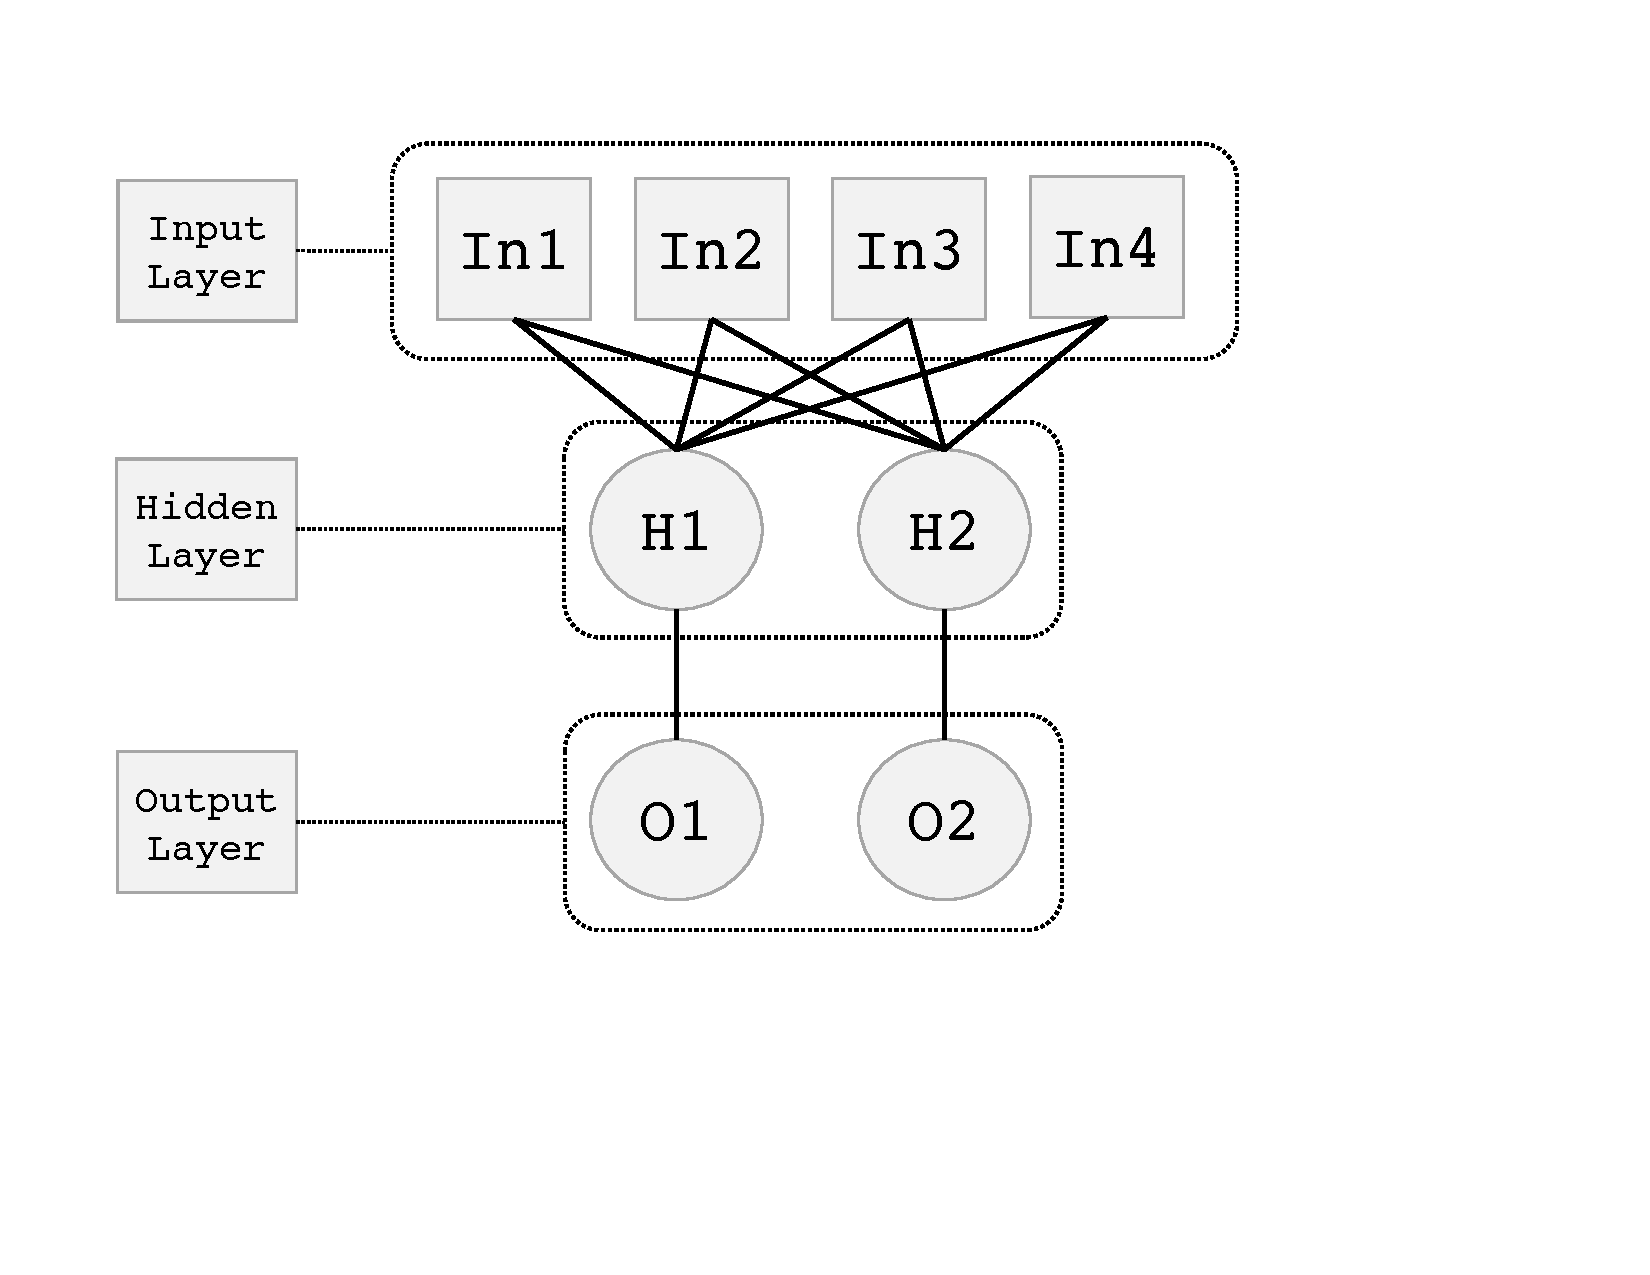
\includegraphics[width=3.5in]{exampleNetwork}
  \end{center}

\vspace{6pt} 
\noindent
The network has 7 nodes.  The four at the top produce input.  The input is passed down to the two hidden-layer
nodes in the middle.  These nodes then do some computation, based upon the neural weights that connect them to
the input layer, and send results to the two output nodes.

\vspace{6pt}
\noindent 
During the training of the network, the output nodes will check whether the output they receive is correct, and
send signals back to the hidden layer accordingly.  Depending upon whether or not the results were correct, the
hidden-layer nodes will adjust the weights that they use in their calculations.  Over time, error will be
reduced, and the network will learn to recognize objects in images based upon their primary color.

\begin{enumerate}
	\item \textbf{Setting Up}:  Each node in the network will consist of a single person.  Alternatively,
		each hidden-layer node can consist of two people, one for doing the feed-forward calculations,
		and one for doing backpropagation weight adjustments.  Similarly, you may have one person doing
		the job of multiple input/output nodes. For instance, if you want all participants to do the
		simulation of hidden-layer nodes, then you can divide the class into two groups, one
		corresponding to \texttt{H1} and one corresponding to \texttt{H2}.  The instructor can then read
		out the vector of inputs for each image, and then tell each group how to compute their error in
		each instance.

		Supplies are handed out as follows:
		\begin{itemize}
			\item Each input neuron receives one of the 4 input (color) cards.
			\item Each hidden-layer neuron receives a hidden-layer worksheet.
			\item Each output neuron receives one of the 2 output (object class) cards.
		\end{itemize}
		The hidden-layer neurons will fill out the first empty row of the worksheet.  For each of the
		\texttt{Input} columns, enter a starting weight.  These should be generated randomly by flipping
		a coin:  if the coin comes up Heads, then enter weight $0.5$;  if the the coin comes up Tails,
		enter $0$. (The right-most two columns are left empty.)

\pagebreak 

\item \textbf{Training}: In the training phase, we cycle through a set of images, and compute a
		response to each of them as follows:
		\begin{itemize}
			\item Each input neuron should look at the image, and then pass on a response to each of
				the hidden-layer neurons.  This response should be $1$ if the image features the
				color for your neuron, and it should be $0$ otherwise.  The hidden-layer neurons
				should write the inputs in the next row, in the appropriate columns.

			\item Each hidden-layer neuron should compute their response to the input.  In each
				case, this will be the weighted sum:
				\[
					R = w_1 \cdot in_1 + w_2 \cdot in_2 + w_3 \cdot in_3 + w_4 \cdot in_4 
				\]
				Write this result in the \texttt{Response} column, and communicate it to the
				single output neuron that is connected to the hidden-layer neuron.

		\item Each output neuron should look at the image.  If the image \textbf{does} contain
				an object to which it responds, then the output neuron 
				computes the \textbf{error}:  the difference between the correct answer and the
				response it received: $E = (1- R)$.  If the images \textbf{does not} contain an
				object to which it responds, the error computed is $E = (0-R)$.

		\item The error results computed by the output neurons are communicated back to their connect
			hidden-layer neurons.  The neurons write this down in the \texttt{Error} column and then
			adjust their 4 input weights as follows, setting each weight as:
			\[
				w_i \leftarrow w_i + (in_i * E)
			\]
			These can be written down in the next row of the worksheet.
		\end{itemize}
	This process repeats until the network is producing correct output on every input.  The time that this
	takes can vary depending upon the randomness of the initial weights, but usually within 2--3 cycles
	through the (small) data-set, the network will have learned its functions, with one neuron detecting all
	apples in the images, and the other all non-apples.

\end{enumerate} 

\end{document}
 
